\chapter{Android Studio}

\section{Estructura de lo proyectos y las carpetas}

En Android Studio, la estructura de un proyecto sigue una convención específica que facilita el desarrollo de aplicaciones Android. Las carpetas y los tipos de archivos más comunes en un proyecto de Android Studio son:

\begin{enumerate}
    \item \texttt{app} Esta carpeta contiene los archivos específicos de la aplicación, incluyendo el código fuente, los recursos y las configuraciones relacionadas.
    \begin{itemize}
        \item \texttt{scr} En esta carpeta se encuentran los archivos del código fuente del proyecto.
        \begin{itemize}
            \item \texttt{scr/main} Código fuente principal de la app
            \begin{itemize}
                \item \texttt{scr/main/java} En esta carpeta se encuentran los archivos de código fuente escritos en lenguaje Java o Kotlin.
                \item \texttt{scr/main/res} Contiene los recursos de la aplicación, como archivos de diseño XML, imágenes y otros recursos estáticos.
                \item \texttt{scr/mainAndroidManifest.xml}  Este archivo es obligatorio y describe la configuración básica de la aplicación, como los componentes, los permisos y las versiones de Android compatibles.
            \end{itemize}
        \end{itemize}
        \item \texttt{build.gradle} Este archivo define la configuración del proyecto y las dependencias utilizadas por la aplicación.
    \end{itemize}
    \item \texttt{gradle} Contiene los archivos de configuración para Gradle, que es la herramienta de compilación utilizada por Android Studio.
    \begin{itemize}
        \item \texttt{gradle/wrapper} Esta carpeta contiene los archivos necesarios para la distribución de Gradle Wrapper, que permite ejecutar Gradle sin necesidad de instalarlo globalmente.
    \end{itemize}
    \item \texttt{build} Contiene los archivos generados después de compilar el proyecto. Los archivos compilados, los recursos procesados y los archivos APK se encuentran aquí.
    \item \texttt{app/build} Aquí se almacenan los archivos generados específicos del módulo de la aplicación, como archivos de compilación, archivos de recursos procesados y el archivo APK final.
    \item \texttt{.idea} Esta carpeta es creada por IntelliJ IDEA (en el cual se basa Android Studio) y contiene archivos de configuración específicos del proyecto.
    \item \texttt{gradle.properties} Este archivo contiene propiedades de configuración para Gradle.
    \item \texttt{settings.gradle}  Aquí se define la configuración global del proyecto, como los módulos incluidos.
\end{enumerate}

La manera en la que Android Studio muestra las diferentes carpetas puede ser distinta a la convención anteriormente mostrada. Cuando se abre un proyecto de Android Studio, la vista de carpetas en el panel izquierdo de la interfaz muestra una estructura simplificada para facilitar la navegación y el desarrollo de la aplicación. Aunque no se muestren todas las carpetas y archivos en la vista de Android Studio, todas las carpetas y archivos mencionados anteriormente (y más) siguen existiendo en el sistema de archivos del proyecto.

La forma en la que se relaciona la estructura con la que Andriod Studio muestra los directorios con la forma en que se encuentran realmente es la siguiente:

\begin{itemize}
    \item \texttt{manifests}  En la vista de Android Studio, esta carpeta contiene el archivo AndroidManifest.xml. El archivo AndroidManifest.xml se encuentra en la ruta \texttt{app/src/main/AndroidManifest.xml} en el sistema de archivos del proyecto.
    \item \texttt{java} En la vista de Android Studio, esta carpeta representa la carpeta \texttt{app/src/main/java} en el sistema de archivos del proyecto. Aquí es donde se encuentra el código fuente de la aplicación en lenguaje Java o Kotlin.
    \item \texttt{res}  En la vista de Android Studio, esta carpeta representa la carpeta \texttt{app/src/main/res} en el sistema de archivos del proyecto. Aquí se encuentran los recursos de la aplicación, como archivos de diseño XML, imágenes y otros recursos estáticos.
\end{itemize}

\section{Entorno Visual}

 La carpeta "res" en Android Studio es una parte fundamental de la estructura de un proyecto, ya que contiene los recursos utilizados por tu aplicación Android. Aquí es donde se almacenan diversos tipos de archivos necesarios para el funcionamiento y la apariencia de la aplicación. 

\begin{itemize}
    \item  drawable: Este directorio contiene los recursos gráficos de tu aplicación, como imágenes, iconos o archivos XML que definen formas y estilos gráficos.
    \item layout: Aquí se encuentran los archivos XML que definen la estructura y el diseño de las interfaces de usuario de tu aplicación. Utilizando el lenguaje de marcado XML, puedes crear y personalizar las vistas y los elementos de la interfaz.
    \item values: En este directorio se almacenan los archivos XML que contienen diferentes valores utilizados en tu aplicación, como cadenas de texto, dimensiones, colores, estilos y temas. Estos archivos permiten centralizar y reutilizar los valores en varios lugares de tu proyecto.
    \item mipmap: Este directorio se utiliza para almacenar los iconos de la aplicación en diferentes densidades de píxeles. Los iconos mipmap se utilizan en el lanzador de la aplicación, en la barra de notificaciones y en otros lugares donde se requieren íconos de alta resolución.
    \item anim: Aquí puedes colocar archivos XML que definen animaciones para tu aplicación, como transiciones, rotaciones o cambios de escala.
    \item menu: En este directorio se encuentran los archivos XML que definen los menús de opciones para tu aplicación. Puedes crear menús con elementos y acciones personalizadas para permitir a los usuarios interactuar con tu aplicación.
\end{itemize}

\subsection{layout} En esta carpeta se almacenan los archivos de descripción XML de las interfaces de usuario. La estructura puede resumirse de la siguiente manera:
\begin{enumerate}
    \item \texttt{activity\_main.xml}: Este es un archivo de ejemplo que se crea de forma predeterminada cuando creas un nuevo proyecto en Android Studio. Representa el diseño de la actividad principal de tu aplicación. La actividad principal es la pantalla principal que se muestra al iniciar la aplicación.
    \item \texttt{fragment\_*.xml}: Los archivos XML con nombres que comienzan con "fragment\_" representan los diseños de los fragmentos utilizados en tu aplicación. Los fragmentos son componentes reutilizables que se pueden combinar y reemplazar dentro de una actividad para crear interfaces de usuario flexibles.
    \item \texttt{item\_*.xml}: Los archivos XML con nombres que comienzan con "item\_" se utilizan en listas o adaptadores para definir el diseño de cada elemento individual de la lista. Por ejemplo, si tienes una lista de elementos en tu aplicación, puedes definir el diseño de cada elemento utilizando un archivo "item\_*.xml".
    \item \texttt{activity\_*.xml}: Los archivos XML con nombres que comienzan con "activity\_" representan los diseños de las actividades adicionales de tu aplicación, aparte de la actividad principal. Cada archivo "activity\_*.xml" define el diseño de una actividad específica de tu aplicación.
\end{enumerate}

En los archivos XML de la carpeta "layout", se puede utilizar elementos y atributos predefinidos, así como crear vistas personalizadas. Se pueden utilizar diferentes tipos de vistas y grupos de diseño (como LinearLayout, RelativeLayout, ConstraintLayout, etc.) para organizar y posicionar las vistas en la interfaz de usuario.

Además de definir la estructura de las vistas, los archivos XML en la carpeta "layout" también pueden incluir atributos para personalizar el aspecto de las vistas, como el tamaño, el color, la fuente, los márgenes y los atributos de comportamiento.

Recuerda que los archivos XML en la carpeta "layout" son solo una parte de la configuración de la interfaz de usuario de tu aplicación. También necesitarás interactuar con ellos en el código Java o Kotlin para asignar comportamientos y manipular los elementos de la interfaz de usuario en tiempo de ejecución.

El diseño se puede describir a través de diferentes grupos de diseño

\subsubsection{\texttt{linearlayout}} Este grupo organiza las vistas en una sola dirección, ya sea horizontal o vertical. Se puede establecer esta dirección utilizando el atributo \texttt{android:orientation} con los valores "\texttt{horizontal}" o "\texttt{vertical}". Las vistas dentro de un LinearLayout se colocan una después de la otra, en el orden en que se definen en el archivo XML. Puedes ajustar la alineación, el espaciado y el peso de las vistas dentro del LinearLayout utilizando atributos adicionales.

Algunos atributos que se pueden usar son:

\begin{enumerate}
\item \texttt{android:orientation}: Define la dirección del \texttt{LinearLayout}. Puede ser \texttt{"horizontal"} para organizar las vistas en una fila horizontal, o \texttt{"vertical"} para organizarlas en una columna vertical.

\item \texttt{android:layout\_width}: Especifica el ancho de la vista. Puede tener valores como \\ \texttt{"wrap\_content"} para ajustarse al contenido de la vista, \texttt{"match\_parent"} para ocupar todo el ancho disponible del contenedor, o un tamaño específico como \texttt{"100dp"}.

\item \texttt{android:layout\_height}: Especifica la altura de la vista. Puede tener valores similares a \texttt{android:layout\_width}.

\item \texttt{android:gravity}: Define la alineación del contenido dentro de la vista. Puede incluir valores como \texttt{"center"}, \texttt{"start"}, \texttt{"end"}, \texttt{"top"}, \texttt{"bottom"}, \texttt{"center\_vertical"}, \texttt{"center\_horizontal"} \ entre otros.

\item \texttt{android:layout\_weight}: Asigna un peso relativo a una vista en un \texttt{LinearLayout}. Puedes utilizarlo para controlar cómo se distribuye el espacio disponible entre las vistas cuando el ancho o el alto es \texttt{wrap\_content}. El valor del peso se utiliza para calcular qué porción del espacio disponible se asigna a cada vista.

\item \texttt{android:layout\_margin}: Establece los márgenes externos de la vista. Puede ser un valor único para aplicar el mismo margen a los cuatro lados, o puedes especificar márgenes diferentes utilizando los atributos \texttt{android:layout\_marginTop}, \ \texttt{android:layout\_marginBottom}, \texttt{android:layout\_marginStart} y \texttt{android:layout\_marginEnd}.
\end{enumerate}


\subsection{Elementos de vista}

\subsubsection{\texttt{<ImageView>}}

Algunos de los atributos que podemos ver en este elemento son:

\begin{enumerate}
\item \texttt{android:src}: Especifica la fuente de la imagen que se mostrará en el ImageView. Puede ser una referencia a un recurso de imagen en el proyecto, como \texttt{"@drawable/mi\_imagen"}, o una URL de una imagen remota.

\item \texttt{android:scaleType}: Define cómo se escala y se ajusta la imagen dentro del ImageView. Se pueden usar valores como \texttt{"centerCrop"}, \texttt{"fitCenter"}, \texttt{"centerInside"}, \texttt{"fitXY"}, entre otros, según las necesidades de diseño.

\item \texttt{android:layout\_width} y \texttt{android:layout\_height}: Estos atributos establecen el ancho y la altura del ImageView. Se pueden utilizar valores como \texttt{"wrap\_content"} para ajustar el tamaño al contenido de la imagen, \texttt{"match\_parent"} para que ocupe todo el ancho o alto disponible del contenedor, o un tamaño específico como \texttt{"100dp"}.

\item \texttt{android:adjustViewBounds}: Este atributo indica si el ImageView debe ajustar su tamaño para mantener las proporciones de la imagen original. Puede ser útil cuando se desea mantener la relación de aspecto de la imagen al cambiar el tamaño del ImageView.

\item \texttt{android:clickable} y \texttt{android:onClick}: Estos atributos permiten hacer que el ImageView sea interactivo. Se puede establecer \texttt{android:clickable="true"} para habilitar la interacción y utilizar \texttt{android:onClick} para especificar el método que se ejecutará cuando se haga clic en el ImageView.

\item \texttt{android:contentDescription}: Proporciona una descripción textual de la imagen para ayudar a los usuarios con discapacidad visual. Es una buena práctica agregar una descripción significativa para cada imagen, especialmente si el ImageView no muestra ningún texto adicional que indique su propósito.
\end{enumerate}

Estos son solo algunos de los atributos más comunes que puedes utilizar en un \texttt{<ImageView>}. Hay otros atributos disponibles, como efectos visuales (\texttt{android:alpha}, \texttt{android:tint}), manipulación de colores (\texttt{android:backgroundTint}, \texttt{android:imageTint}), entre otros. Puedes consultar la documentación oficial de Android para obtener una lista completa de todos los atributos disponibles para \texttt{<ImageView>} y sus descripciones detalladas.



\subsection{values}

Dentro de la carpeta de recursos se puede crear una carpeta adicional para declarar algunas variables que indiquen valores a los cuales se puede acceder desde las descripciones de las vistas.

\begin{figure}[H]
    \centering
    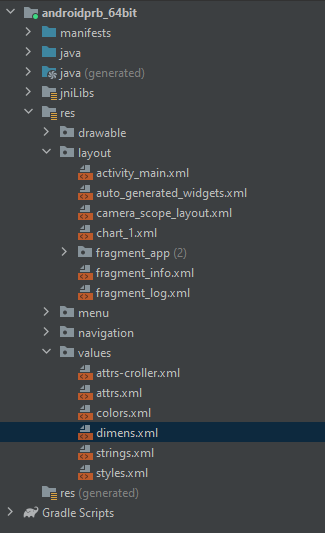
\includegraphics[scale=0.5]{android_apps/android_f1.png}
\end{figure}

dentro del archivo \texttt{dimens.xml} se encuentran las siguientes declaraciones: \newpage

\begin{verbatim}
<resources>
    <!-- Default screen margins, per the Android Design guidelines. -->
    <dimen name="activity_horizontal_margin">16dp</dimen>
    <dimen name="activity_vertical_margin">16dp</dimen>
    <dimen name="fab_margin">16dp</dimen>
    <dimen 
        name="appbar_padding">8dp</dimen>
    <dimen 
        name="appbar_padding_top">8dp</dimen>
    <dimen name="appname_bar_height">30dp</dimen>
    <dimen name="appname_textsize">20dp</dimen>
    <dimen name="info_cardview_margin">10dp</dimen>
    <dimen name="info_linear_padding">20dp</dimen>
    <dimen name="divider_height">2dp</dimen>
    <dimen name="info_sectiondata_paddingtop">5dp</dimen>
    <dimen name="info_sectiontitle_paddingbottom">10dp</dimen>
    <dimen name="uimarginbottom">8dp</dimen>
</resources>
\end{verbatim}

Y dentro de los \texttt{views} se pueden referir a estas variables mediante la siguiente forma: \\

\texttt{android:layout\_height="@dimen/appname\_bar\_height"}